\documentclass[a4paper,12pt,twoside,swedish]{report}

%\graphicspath{{figures/}}

%Inkluderar olika paket
\usepackage{times}  
\usepackage{amsmath}
\usepackage{amssymb}
\usepackage{graphicx}
\usepackage{theorem}
\usepackage[latin1]{inputenc}
\usepackage{latexsym}
\usepackage{url}
\usepackage{babel}
\usepackage{titlesec}
\usepackage[affil-it]{authblk}

\headsep          0.25in
\headheight       12pt
\setlength{\topmargin}{-\headsep}
\addtolength{\topmargin}{-\headheight}
\oddsidemargin      0in
\evensidemargin     0in
\setlength{\textwidth}{\paperwidth}
\addtolength{\textwidth}{-2.0in}
\setlength{\textheight}{\paperheight}
\addtolength{\textheight}{-2.0in}
\addtolength{\textheight}{-1\topskip}
\divide\textheight  by \baselineskip
\multiply\textheight  by \baselineskip
\addtolength{\textheight}{\topskip}

\addto\captionsswedish{
  \renewcommand{\contentsname}
    {Inneh�llsf�rteckning}
}

%F�r att f� bra numrering och inte att det ska st� Kapitel 1
\titleformat{\chapter}
  {\Large\bfseries} % format
  {}                % label
  {0pt}             % sep
  {\huge}           % before-code
%

\begin{document}

\pagestyle{empty}

%----------------------------- Front matter of the document

%Framsidan
\title{Simulering av Elastiska Material}
%\date{}
\author{Kalle Bladin\\Erik Broberg\\Emma Forsling Parborg\\Martin Gr�d}

\affil{Link�pings Universitet}
\maketitle

%Sammanfattning
\begin{abstract}
H�r ska sammanfattningen skrivas in
\vfill
\end{abstract}

%Inneh�llsf�rteckning, Figurer, Tabeller
\tableofcontents  % chapter with the table of contents
\addtocontents{toc}{\protect\thispagestyle{empty}}
\listoffigures    % chapter with the list of figures
\addtocontents{lof}{\protect\thispagestyle{empty}}
\listoftables     % chapter with the list of tables
\addtocontents{lot}{\protect\thispagestyle{empty}}

%----------------------------- Body of the document
\pagestyle{plain}

%1. Inledning
\chapter{Inledning}
Inledande text �r alltid lite trevligt
\setcounter{page}{1}

  \section{Syfte}
  Ett syfte �r sitter aldrig fel det med.

% 2. Metod
\chapter{Metod}
Inledningstext f�r metoden
  \section{Kraftekvationen} 
  �h den var s� kraftig
  
  \section{Matlab}
  Ett annat ord f�r matsal
  
  \section{C++ osv.}
  men nu h�nder de riktiga grejerna

% 3. Resultat
\chapter{Resultat}
WOW, n�men vad trevlig ;) \\Dags att byta rad\\ Byta stycke\\\\nu g�r det bra det h�r

% 4. Diskussion
\chapter{Diskussion}
Nja men nu g�r det v�ll lite �verstyr


% Lite LATEX-kommandon
\chapter{Exempel fr�n Anna}

%Punktlista
\section{Punktlista och n�got mysko}
H�r kommer nu en punktlista skapas
\begin{itemize}
  \item In Catilinam I
  \item In Catilinam II
  \item In Catilinam III
  \item In Catilinam IV
\end{itemize}
Var den inte fin.\\
Vet inte riktigt vad detta g�r?\\
liberis cogitate \cite{AbTaRu:54},  \cite{Abl:56}, \cite{Keo:58} and \cite{Pow:85}. 

%Tabeller
\section{Tabeller}
Nu ska jag skapa en UNDERBAR tabell.\\ 
Jag kan ju till och med referera till den.(\ref{table_example}) %verkar dock lite buggig, blir ? d� och d�
\begin{table}[htbp]
    \caption{Heading centred.}
    \label{table_example}
    \begin{tabular*}{\hsize}{lllll}
      \hline %streck
      Emma & Martin & Kalle & Erik & XXXX\\
      Forsling & Gr�d & Bladin & Broberg & xxxx  \\
      \hline
      X     & X     &      & XXX   &       \\
      XX    & XXX   & XX   & X     & XX    \\
      XXX   & X     & X    & XXX   & XXX   \\
      XXXX  & XX    &      & XX    & X     \\
      X XX  & XXX   & XX   & XXX   & XXXXX \\
      \hline
    \end{tabular*}
\end{table}

%Bilder
\section{Figurer/Bilder}
\begin{figure}
  \begin{center}
    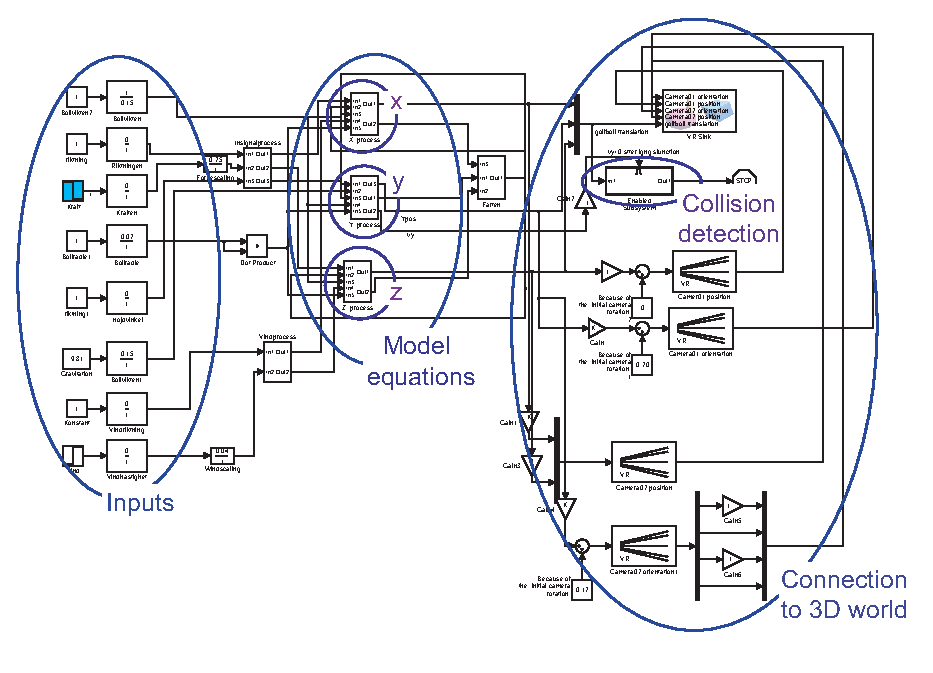
\includegraphics[width=11cm]{Figures/block_simulink.eps} 
  \end{center}
  \caption{Example of figure}
  \label{model_block}
\end{figure}

Figure \ref{model_block} is not by Cicero.

%Ekvationer
\section{Ekvationer}
Some words might be appropriate describing equation \ref{e1}, if we
had but time and space enough.

\begin{equation}
  \frac{\partial F}{\partial
  t}=D\frac{\partial^2 F}{\partial x^2},
  \label{e1}
\end{equation}
%Vet inte riktigt vad denna v�g ska g�ra? Och sen �r det bara massor text och lite till bilder ekvationer
%Kanske har med referenser att g�ra men hittar inte det i dokumentet!!!!!

Ti.~Gracchus, quod iterum tribunus plebis fieri voluit, non
C.~Gracchus, quod agrarios concitare conatus est, non L.~Saturninus,
quod C.~Memmium occidit, in discrimen aliquod atque in vestrae
severitatis iudicium adduciturtenentur ii, qui ad urbis incendium, ad
vestram omnium caedem, ad Catilinam accipiendum Romae restiterunt,
tenentur litterae, signa, manus, denique unius cuiusque confessio;
sollicitantur Allobroges, servitia excitantur, Catilina accersitur; id
est initum consilium, ut interfectis omnibus nemo ne ad deplorandum
quidem populi Romani nomen atque ad lamentandam tanti imperii
calamitatem relinquatur.

Haec omnia indices detulerunt, rei confessi sunt, vos multis iam iudiciis
iudicavistis, primum quod mihi gratias egistis singu laribus verbis et
mea virtute atque diligentia perditorum hominum coniurationem patefactam
esse decrevistis, deinde quod P.~Lentulum se abdicare praetura
coegistis, tum quod eum et ceteros, de quibus iudicastis, in custodiam
dandos censuistis, maximeque quod meo nomine supplicationem decrevistis,
qui honos togato habitus ante me est nemini; postremo hesterno die
praemia legatis Allobrogum Titoque Volturcio dedistis amplissima. Quae
sunt omnia eius modi, ut ii, qui in custodiam nominatim dati sunt, sine
ulla dubitatione a vobis damnati esse videantur.

\section{A section}
Also containing some text, and a figure (\ref{fig:plot_result}).
\begin{figure}
 \begin{center}
   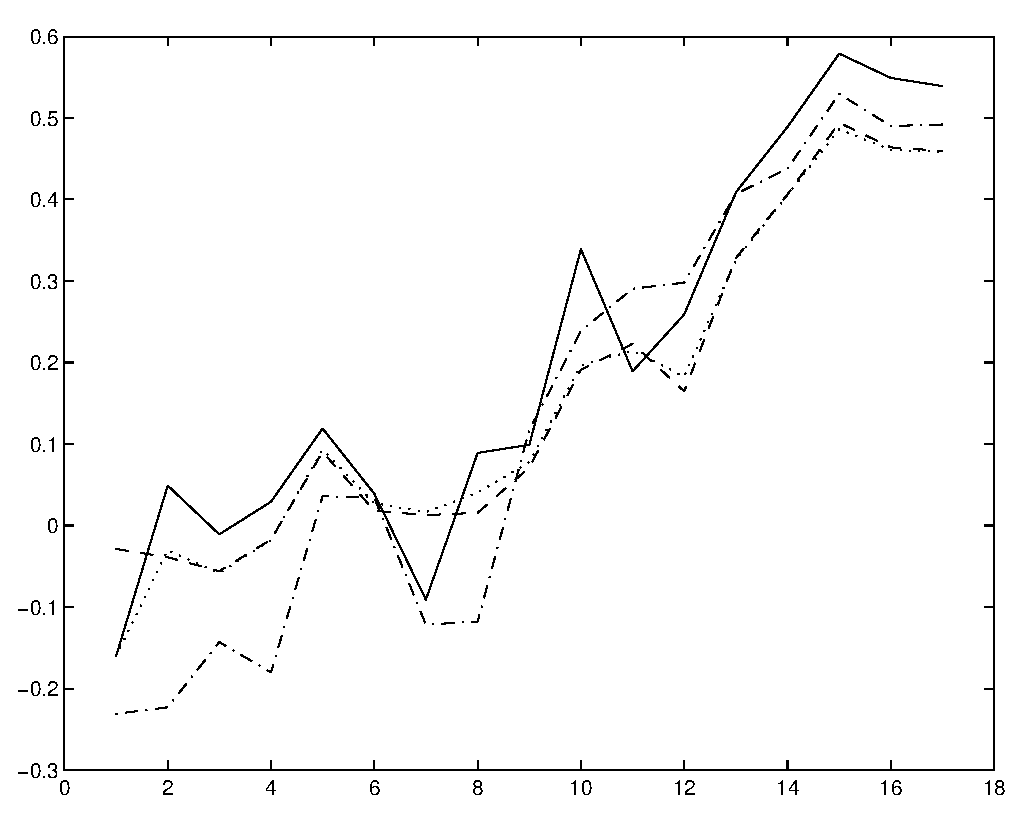
\includegraphics[width=7cm]{Figures/result.eps}  
  \end{center}
\caption{Another figure example}
   \label{fig:plot_result}
\end{figure}

\section{Epilogue}
A word or two to conclude,  and this even includes some
inline maths: \(R(x,t)\sim
t^{-\beta}g(x/t^\alpha)\exp(-|x|/t^\alpha)\)

\subsection{Last words}
 Quae cum ita sint, pro imperio, pro exercitu, pro provincia, quam
neglexi, pro triumpho ceterisque laudis insignibus, quae sunt a me
propter urbis vestraeque salutis custodiam repudiata, pro clientelis
hospitiisque provincialibus, quae tamen urbanis opibus non minore labore
tueor quam comparo, pro his igitur omnibus rebus, pro meis in vos
singularibus studiis proque hac, quam perspicitis, ad conservandam rem
publicam diligentia nihil a vobis nisi huius temporis totiusque mei
consulatus memoriam postulo; quae dunn erit in vestris fixa mentibus,
tutissimo me muro saeptum esse arbitrabor. Quodsi meam spem vis
inproborum fefellerit atque superaverit, commendo vobis parvum meum
filium, cui profecto satis erit praesidii non solum ad salutem, verum
etiam ad dignitatem, si eius, qui haec omnia suo solius periculo
conservarit, illum filium esse memineritis.

\subsection{The very last words}
Quapropter de summa salute
vestra populique Romani, de vestris coniugibus ac liberis, de aris ac
focis, de fanis atque templis de totius urbis tectis ac sedibus, de
imperio ac libertate, de salute Italiae, de universa re publica
decernite diligenter, ut instituistis, ac fortiter. Habetis eum
consulem, qui et parere vestris decretis non dubitet et ea \cite{fortran}, quae
statueritis, quoad vivet, defendere et per se ipsum praestare possit.

%----------------------------- Back matter of the document

\bibliographystyle{vancouver}
\bibliography{bibsam}

\addcontentsline{toc}{chapter}{Litteraturf�rteckning}

\pagestyle{empty}

\appendix

\chapter{Proof of\dots}

\label{app:proof1}

\thispagestyle{empty}

Proof\dots

Quare, patres conscripti, consulite vobis, prospicite patriae,
conservate vos, coniuges, liberos fortunasque vestras, populi Romani
nomen salutemque defendite; mihi parcere ac de me cogitare desinite. Nam
primum debeo sperare omnis deos, qui huic urbi praesident, pro eo mihi,
ac mereor, relaturos esse gratiam; deinde, si quid obtigerit, aequo
animo paratoque moriar. Nam neque turpis mors forti viro potest accidere
neque immatura consulari nec misera sapienti. Nec tamen ego sum ille
ferreus, qui fratris carissimi atque amantissimi praesentis maerore non
movear horumque omnium lacrumis, a quibus me circumsessum videtis Neque
meam mentem non domum saepe revocat exanimata uxor et abiecta metu filia
et parvulus filius quem mihi videtur amplecti res publica tamquam ob
sidem consulatus mei, neque ille, qui expectans huius exitum diei stat
in conspectu meo, gener. Moveo his rebus omnibus, sed in eam partem, uti
salvi sint vobiscum omnes, etiamsi me vis aliqua oppresserit, potius,
quam et illi et nos una rei publicae peste pereamus.

Quare, patres conscripti, incumbite ad salutem rei publicae,
circumspicite omnes procellas, quae inpendent, nisi providetis. Non
Ti.~Gracchus, quod iterum tribunus plebis fieri voluit, non
C.~Gracchus, quod agrarios concitare conatus est, non L.~Saturninus,
quod C.~Memmium occidit, in discrimen aliquod atque in vestrae
severitatis iudicium adduciturtenentur ii, qui ad urbis incendium, ad
vestram omnium caedem, ad Catilinam accipiendum Romae restiterunt,
tenentur litterae, signa, manus, denique unius cuiusque confessio;
sollicitantur Allobroges, servitia excitantur, Catilina accersitur; id
est initum consilium, ut interfectis omnibus nemo ne ad deplorandum
quidem populi Romani nomen atque ad lamentandam tanti imperii
calamitatem relinquatur.Quare, patres conscripti, consulite vobis, prospicite patriae,
conservate vos, coniuges, liberos fortunasque vestras, populi Romani
nomen salutemque defendite; mihi parcere ac de me cogitare desinite. Nam
primum debeo sperare omnis deos, qui huic urbi praesident, pro eo mihi,
ac mereor, relaturos esse gratiam; deinde, si quid obtigerit, aequo
animo paratoque moriar. Nam neque turpis mors forti viro potest accidere
neque immatura consulari nec misera sapienti. Nec tamen ego sum ille
ferreus, qui fratris carissimi atque amantissimi praesentis maerore non
movear horumque omnium lacrumis, a quibus me circumsessum videtis Neque
meam mentem non domum saepe revocat exanimata uxor et abiecta metu filia
et parvulus filius quem mihi videtur amplecti res publica tamquam ob
sidem consulatus mei, neque ille, qui expectans huius exitum diei stat
in conspectu meo, gener. Moveo his rebus omnibus, sed in eam partem, uti
salvi sint vobiscum omnes, etiamsi me vis aliqua oppresserit, potius,
quam et illi et nos una rei publicae peste pereamus.

Quare, patres conscripti, incumbite ad salutem rei publicae,
circumspicite omnes procellas, quae inpendent, nisi providetis. Non
Ti.~Gracchus, quod iterum tribunus plebis fieri voluit, non
C.~Gracchus, quod agrarios concitare conatus est, non L.~Saturninus,
quod C.~Memmium occidit, in discrimen aliquod atque in vestrae
severitatis iudicium adduciturtenentur ii, qui ad urbis incendium, ad
vestram omnium caedem, ad Catilinam accipiendum Romae restiterunt,
tenentur litterae, signa, manus, denique unius cuiusque confessio;
sollicitantur Allobroges, servitia excitantur, Catilina accersitur; id
est initum consilium, ut interfectis omnibus nemo ne ad deplorandum
quidem populi Romani nomen atque ad lamentandam tanti imperii
calamitatem relinquatur.Quare, patres conscripti, consulite vobis, prospicite patriae,
conservate vos, coniuges, liberos fortunasque vestras, populi Romani
nomen salutemque defendite; mihi parcere ac de me cogitare desinite. Nam
primum debeo sperare omnis deos, qui huic urbi praesident, pro eo mihi,
ac mereor, relaturos esse gratiam; deinde, si quid obtigerit, aequo
animo paratoque moriar. Nam neque turpis mors forti viro potest accidere
neque immatura consulari nec misera sapienti. Nec tamen ego sum ille
ferreus, qui fratris carissimi atque amantissimi praesentis maerore non
movear horumque omnium lacrumis, a quibus me circumsessum videtis Neque
meam mentem non domum saepe revocat exanimata uxor et abiecta metu filia
et parvulus filius quem mihi videtur amplecti res publica tamquam ob
sidem consulatus mei, neque ille, qui expectans huius exitum diei stat
in conspectu meo, gener. Moveo his rebus omnibus, sed in eam partem, uti
salvi sint vobiscum omnes, etiamsi me vis aliqua oppresserit, potius,
quam et illi et nos una rei publicae peste pereamus.

\chapter{Second proof of\dots}

\label{app:proof2}

\thispagestyle{empty}


Quare, patres conscripti, incumbite ad salutem rei publicae,
circumspicite omnes procellas, quae inpendent, nisi providetis. Non
Ti.~Gracchus, quod iterum tribunus plebis fieri voluit, non
C.~Gracchus, quod agrarios concitare conatus est, non L.~Saturninus,
quod C.~Memmium occidit, in discrimen aliquod atque in vestrae
severitatis iudicium adduciturtenentur ii, qui ad urbis incendium, ad
vestram omnium caedem, ad Catilinam accipiendum Romae restiterunt,
tenentur litterae, signa, manus, denique unius cuiusque confessio;
sollicitantur Allobroges, servitia excitantur, Catilina accersitur; id
est initum consilium, ut interfectis omnibus nemo ne ad deplorandum
quidem populi Romani nomen atque ad lamentandam tanti imperii
calamitatem relinquatur.Quare, patres conscripti, consulite vobis, prospicite patriae,
conservate vos, coniuges, liberos fortunasque vestras, populi Romani
nomen salutemque defendite; mihi parcere ac de me cogitare desinite. Nam
primum debeo sperare omnis deos, qui huic urbi praesident, pro eo mihi,
ac mereor, relaturos esse gratiam; deinde, si quid obtigerit, aequo
animo paratoque moriar. Nam neque turpis mors forti viro potest accidere
neque immatura consulari nec misera sapienti. Nec tamen ego sum ille
ferreus, qui fratris carissimi atque amantissimi praesentis maerore non
movear horumque omnium lacrumis, a quibus me circumsessum videtis Neque
meam mentem non domum saepe revocat exanimata uxor et abiecta metu filia
et parvulus filius quem mihi videtur amplecti res publica tamquam ob
sidem consulatus mei, neque ille, qui expectans huius exitum diei stat
in conspectu meo, gener. Moveo his rebus omnibus, sed in eam partem, uti
salvi sint vobiscum omnes, etiamsi me vis aliqua oppresserit, potius,
quam et illi et nos una rei publicae peste pereamus.

Quare, patres conscripti, incumbite ad salutem rei publicae,
circumspicite omnes procellas, quae inpendent, nisi providetis. Non
Ti.~Gracchus, quod iterum tribunus plebis fieri voluit, non
C.~Gracchus, quod agrarios concitare conatus est, non L.~Saturninus,
quod C.~Memmium occidit, in discrimen aliquod atque in vestrae
severitatis iudicium adduciturtenentur ii, qui ad urbis incendium, ad
vestram omnium caedem, ad Catilinam accipiendum Romae restiterunt,
tenentur litterae, signa, manus, denique unius cuiusque confessio;
sollicitantur Allobroges, servitia excitantur, Catilina accersitur; id
est initum consilium, ut interfectis omnibus nemo ne ad deplorandum
quidem populi Romani nomen atque ad lamentandam tanti imperii
calamitatem relinquatur.Quare, patres conscripti, consulite vobis, prospicite patriae,
conservate vos, coniuges, liberos fortunasque vestras, populi Romani
nomen salutemque defendite; mihi parcere ac de me cogitare desinite. Nam
primum debeo sperare omnis deos, qui huic urbi praesident, pro eo mihi,
ac mereor, relaturos esse gratiam; deinde, si quid obtigerit, aequo
animo paratoque moriar. Nam neque turpis mors forti viro potest accidere
neque immatura consulari nec misera sapienti. Nec tamen ego sum ille
ferreus, qui fratris carissimi atque amantissimi praesentis maerore non
movear horumque omnium lacrumis, a quibus me circumsessum videtis Neque
meam mentem non domum saepe revocat exanimata uxor et abiecta metu filia
et parvulus filius quem mihi videtur amplecti res publica tamquam ob
sidem consulatus mei, neque ille, qui expectans huius exitum diei stat
in conspectu meo, gener. Moveo his rebus omnibus, sed in eam partem, uti
salvi sint vobiscum omnes, etiamsi me vis aliqua oppresserit, potius,
quam et illi et nos una rei publicae peste pereamus.



Quare, patres conscripti, incumbite ad salutem rei publicae,
circumspicite omnes procellas, quae inpendent, nisi providetis. Non
Ti.~Gracchus, quod iterum tribunus plebis fieri voluit, non
C.~Gracchus, quod agrarios concitare conatus est, non L.~Saturninus,
quod C.~Memmium occidit, in discrimen aliquod atque in vestrae
severitatis iudicium adduciturtenentur ii, qui ad urbis incendium, ad
vestram omnium caedem, ad Catilinam accipiendum Romae restiterunt,
tenentur litterae, signa, manus, denique unius cuiusque confessio;
sollicitantur Allobroges, servitia excitantur, Catilina accersitur; id
est initum consilium, ut interfectis omnibus nemo ne ad deplorandum
quidem populi Romani nomen atque ad lamentandam tanti imperii
calamitatem relinquatur.


\end{document}

